\chapter{Results}

Using training data depicted in figure \ref{fig:head_final_triplet_augmented_collage_1}, we trained the neural network for 72 hours on a NVIDIA K40 \ac{GPU} in the \ac{CSC} Taito computing cluster. The original dataset of 100 000 different rendered images was heavily augmented and looped over numerous times. In total, the network saw over 8 million samples during the training. The final model had 43.7 million parameters taking up 175 megabytes of memory. Rotations were left out from the augmentations because they would have necessitated a substantial increase in the network parameter count.

\section{Real-world images}

We evaluated the network using selected images from the CelebA dataset \cite{liu2015faceattributes}. Feeding one image through the model took on average 17 ms on a NVIDIA GTX 980 \ac{GPU} and 750 ms on an Intel Core i5-3570K \ac{CPU}. In figure \ref{fig:results_1}, from the left, the first image is the input for the network. Next three are the outputs: \textit{result mask}, \textit{occluded result mask}, and \textit{result UV}. The last four images are different visualizations created using the input image and network outputs.

Looking at the \textit{result mask} column in figure \ref{fig:results_1}, it is evident that the network was able to do the segmentation well. That is, the model detected what pixels belong to a human face and what pixels to the background. \textit{Result mask occluded} column shows what the network thought is part of a human face but under some occlusion. The masks were not binary as they had some grayscale values. They were most likely caused by our occlusion augmentation method that sometimes generated transparent occlusion masks. Glasses, sunglasses, hats, hair, beards, and mustaches were detected, even though our training data did not have any of them. In some cases, e.g., with the image of Angela Merkel, the occluded result mask was more accurate than the actual result mask. The network was having some trouble especially when hair was occluding the forehead.

\begin{figure}[p]
    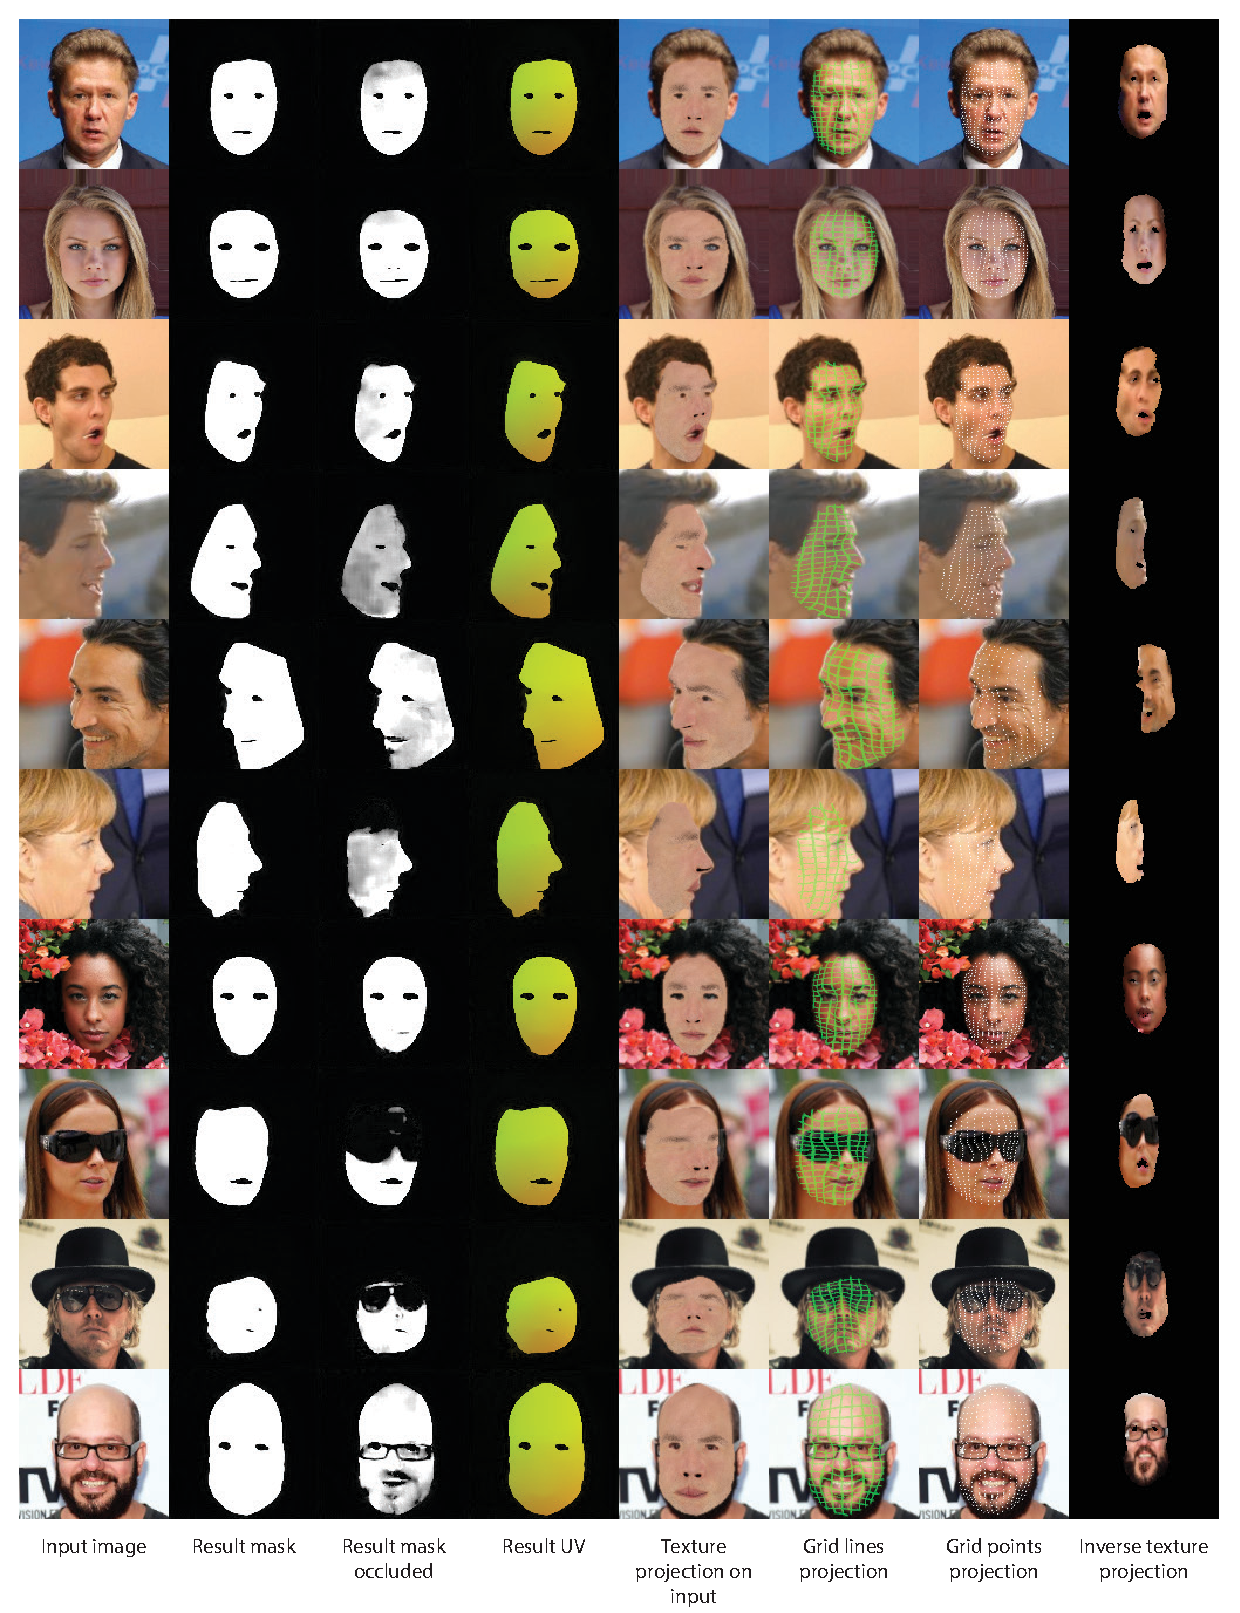
\includegraphics[width=\textwidth]{results1}
    \caption[Real image results]{Results obtained when the network was applied to real-world images. Leftmost image is the input, and the next three are the outputs of the network. Last four images are all visualizations created using the input image and the network outputs.}
    \label{fig:results_1}
\end{figure}

\begin{figure}[p]
    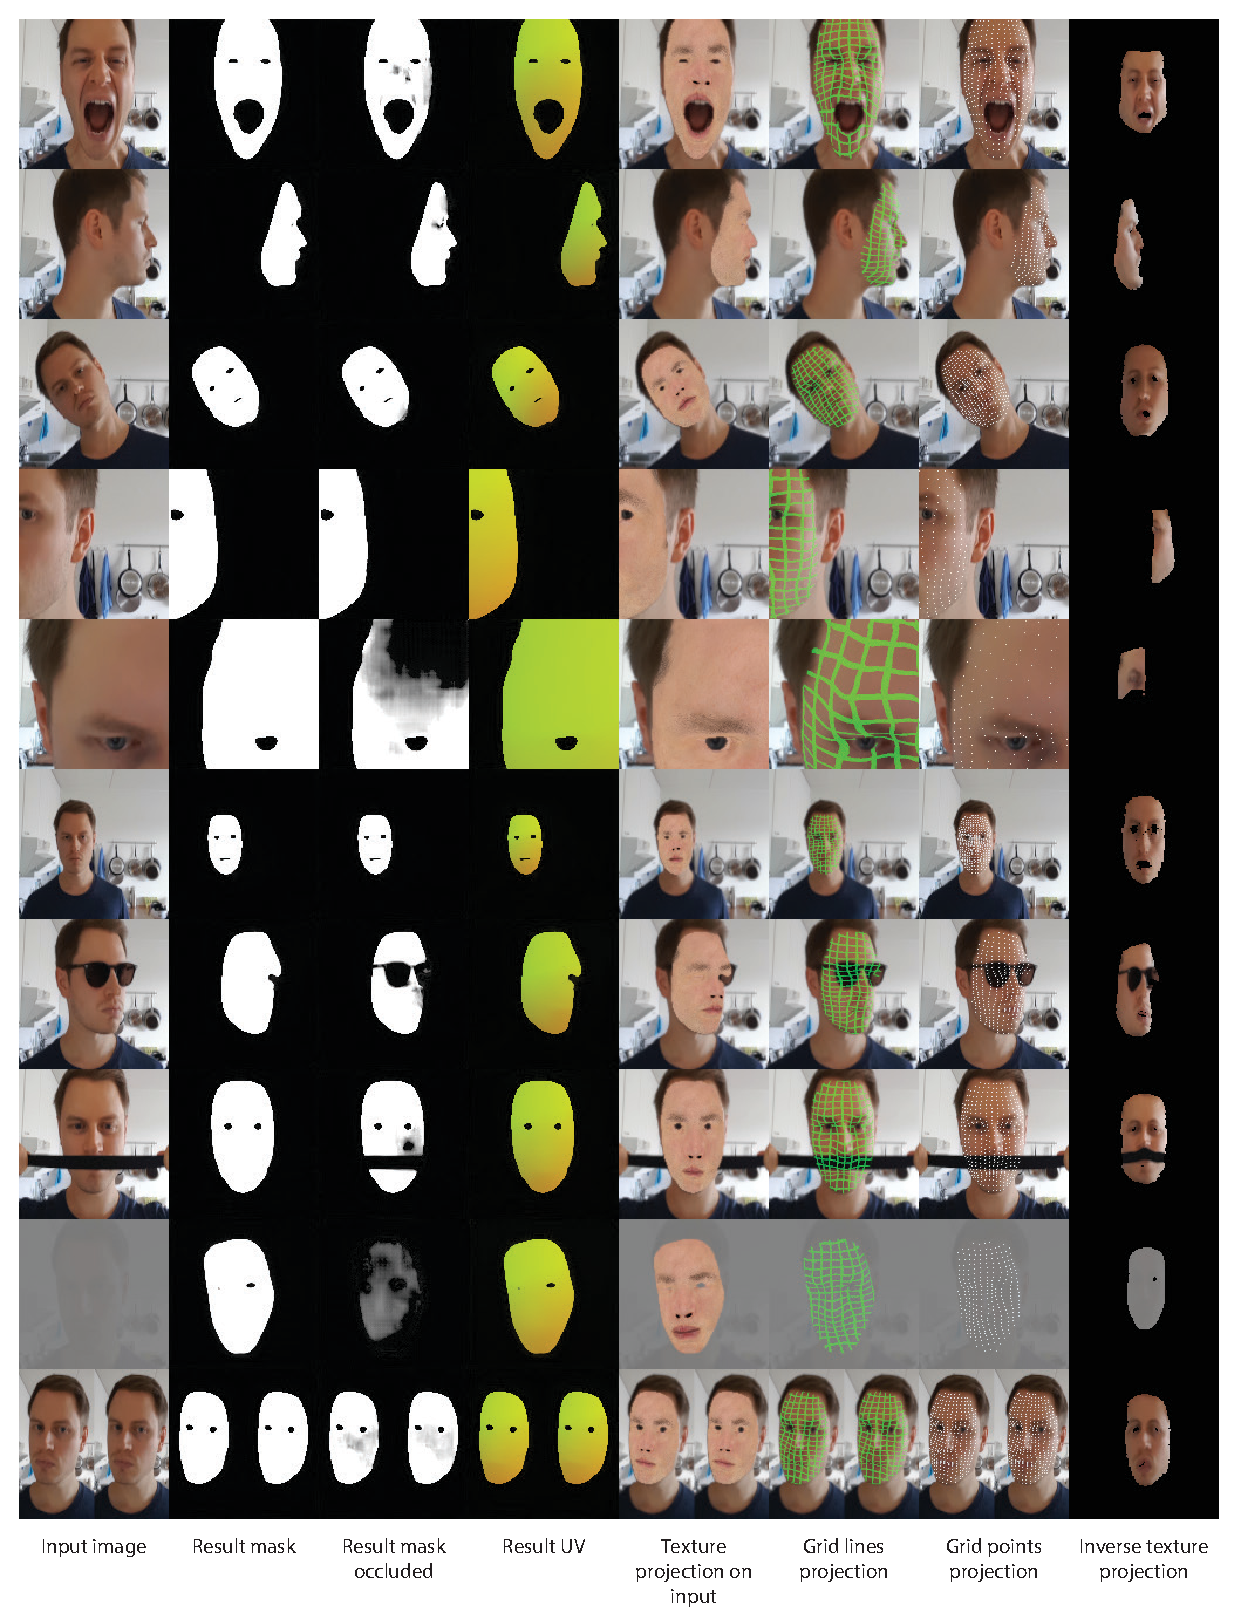
\includegraphics[width=\textwidth]{results2}
    \caption[More real image results]{Results obtained when the network was applied to real-world images with more extreme variations.}
    \label{fig:results_2}
\end{figure}

The \textit{result UV} column in figure \ref{fig:results_1} shows the actual geometry mapping in the UV space generated by the network. Looking at it does not tell too much, other than that the results look about the same as in the training data. But when applied by doing a \textit{texture projection on input}, it is revealed that the geometry mapping worked, and the network was able to track diverse human faces. The second and fifth rows have very different facial geometries, but the texture projections show that the model was able to differentiate between them. The \textit{grid lines projection} shows the geometric contours of the mapping generated by the network. Together with \textit{grid points projection} these two are not that useful with static images but are very good at determining the stability and accuracy of the tracking when applied to a video. The last column shows the \textit{inverse texture projection} where the facial area of the input image is projected into UV domain using the \textit{result UV} mapping. If processed over time and multiple input images, this could be used to generate a texture from the person pictured.

More extreme situations are illustrated in figure \ref{fig:results_2}. The training data did contain expressions with wide open mouths, but not as extreme expressions as in the first row. It shows that the network was able to track a little beyond the training data. Tracking of the face was not lost even at close to right angles, but other disturbances were not well tolerated in these situations. Rendered data contained faces with at most 45-degree angles along the z-axis (out of the paper), and the network was not able to map decent geometries much beyond that. The model worked well even if the subject was halfway out of the frame in any direction. Also, zooming in very close did not pose too much trouble for the network. If the person moved too far away from the camera, the tracking became quickly very unstable. This was mostly caused by the small 128x128 resolution of the input images. The face needed to occupy about one-fourth of the image for successful detection.

Inpainting geometry under the occlusions worked decently. The seventh and eight rows in figure \ref{fig:results_2} show typical results when input images had occlusions. The network detected the occlusions well and was able to generate dense geometry mapping underneath. The problem was that there was usually some warping of the geometry, mouth and eye holes disappeared randomly, and the geometry was not stable. These were most evident when tracking videos with moving occlusions over the faces.

Large variations in brightness and contrast in the input images did not pose problems for the model. Brightness or contrast could be tuned to such extremes that it was difficult for a human to recognize the image. Nevertheless, the network segmented and tracked the faces successfully. In spite of the fact that the training data only contained images with one head, the model was able to differentiate between at least four different faces in one image. There probably is no limit on the number, the only limiting factor, in this case, was the resolution of the input image.

\section{Synthetic images}

\begin{figure}[p]
    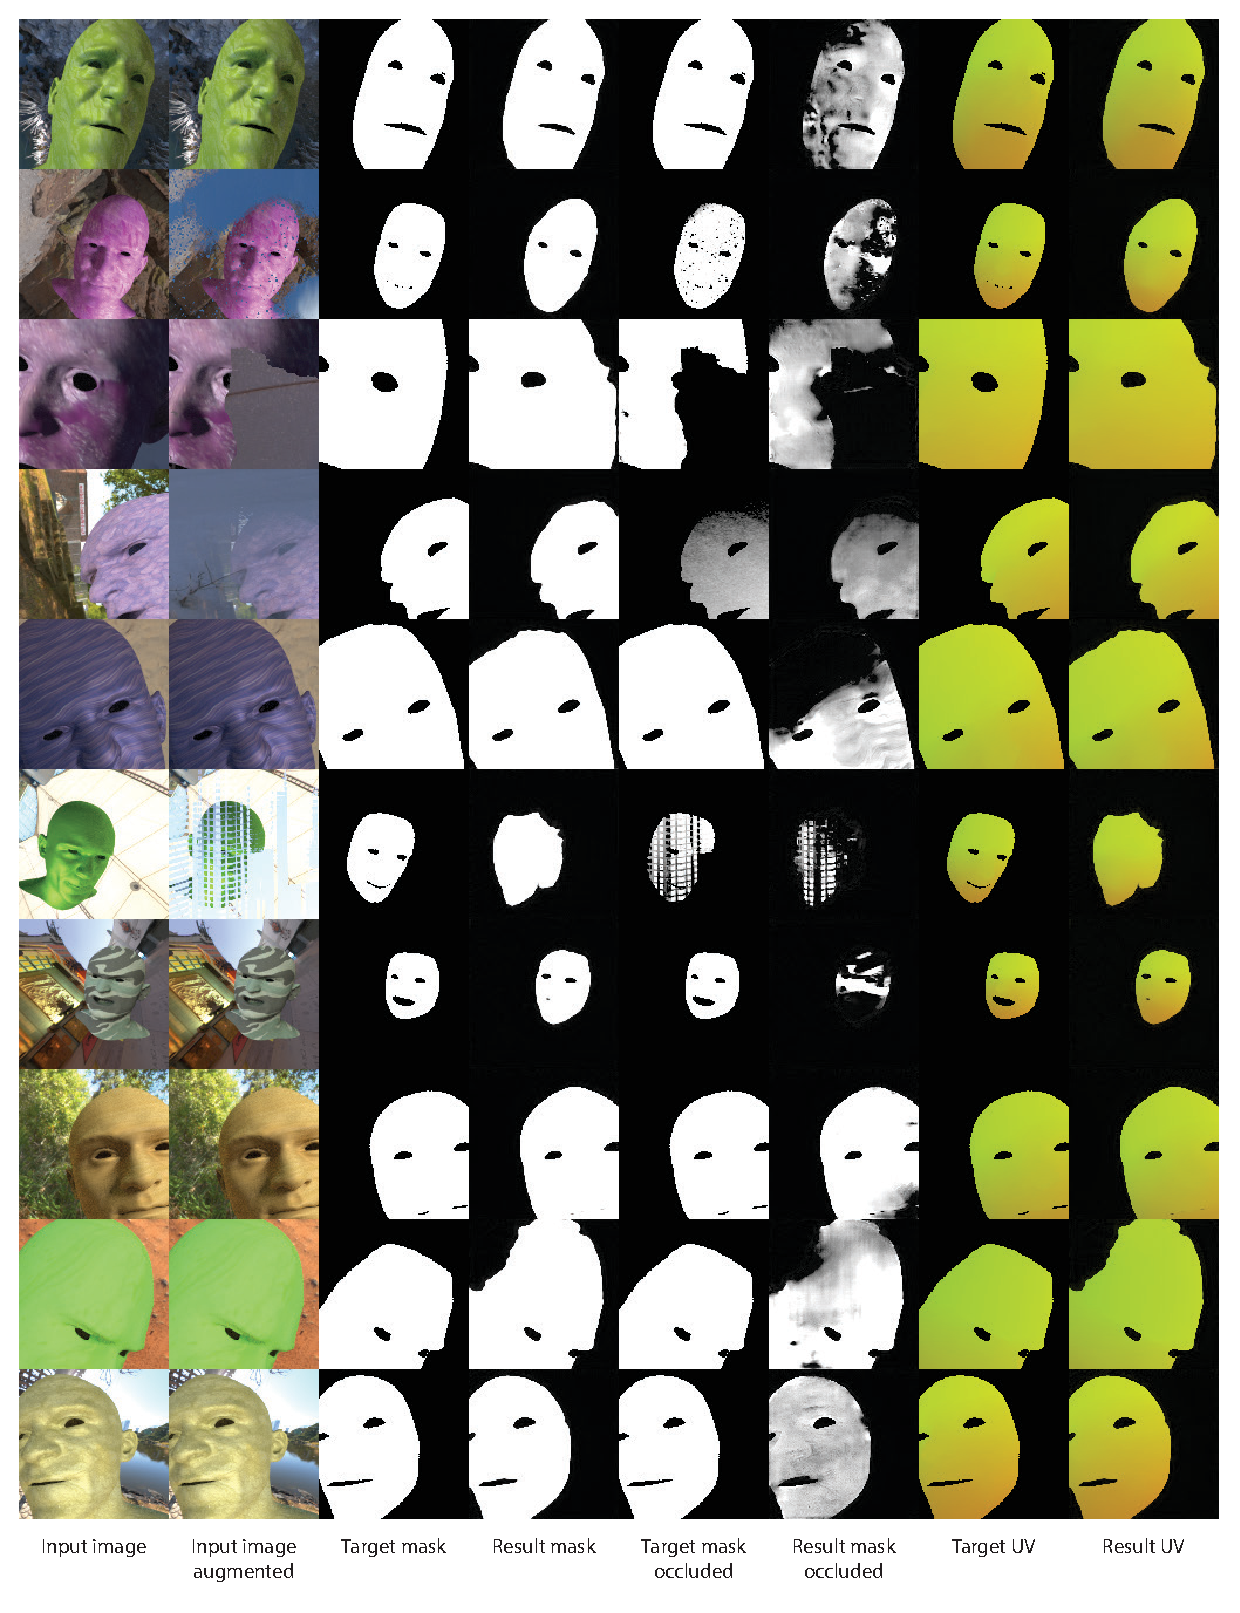
\includegraphics[width=\textwidth]{results3}
    \caption[Synthetic image results]{Results obtained when the network was applied to synthetic and augmented test images. The second, augmented image, was fed to the network. The result images can then be compared with the ground truth target images.}
    \label{fig:results_3}
\end{figure}

Figure \ref{fig:results_3} shows what happened when we fed the network with similar images we used in training. These images were from the test set; the model had not seen these before. The leftmost image is the original render and the second is the original render augmented with every augmentation except rotations. Then there are pairs of target and result images. Target images are the known ground truths, and the result images can be compared with them. The model worked well as it was able to segment faces from the backgrounds and detect occlusions even in some extreme cases. Sometimes it was hard even for humans to recognize faces from the augmented images but the network was able to segment them and generate believable geometry.

\section{Video}

\begin{figure}
    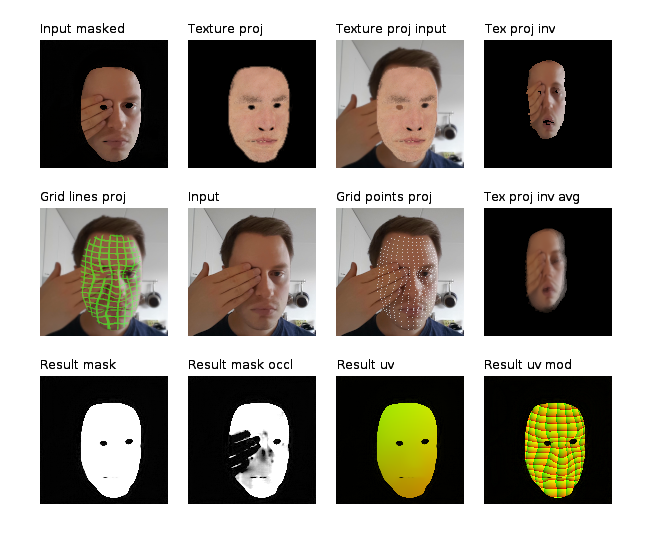
\includegraphics[width=\textwidth]{video_frame}
    \caption[Video result frame]{A frame capture from the test video. Full videos, which can be used to assess the temporal stability of the tracking, are available on YouTube \cite{uvnet}.}
    \label{fig:video_frame_1}
\end{figure}

To assess the temporal stability of the geometry tracking, i.e., it does not vibrate or warp too much over time, we created a test video containing various difficult scenarios. This video can be viewed on YouTube \cite{uvnet}, and a sample frame from the video is shown in figure \ref{fig:video_frame_1}. Grid lines projection and grid points projection were most helpful when evaluating the temporal stability of the results. The video confirmed that the network could be applied to a video with satisfactory results. Temporal stability was good when the movement was slow, and the face was well visible without extreme expressions. As soon as the subject tilted too much away from the camera or their expression was exaggerated, the tracking started to vibrate or even warp to completely wrong geometries. Moving occlusions presented big challenges as the inpainted geometry in these cases was not stable. If there were no subject in the frame, the subject was too far away, the subject was turned away, or their face was occluded, the network tended to ''explode.`` That means that the network output wildly wrong and rapidly changing results instead of just generating black.

\section{Discussion}

The main research problem was whether it is possible to train a neural network using synthetic data to do dense human facial geometry tracking in the real world. We confirmed that it is feasible to train a fully convolutional neural network with skip connections using non-realistic rendered training data and the resulting model generalized to real-world images. Two important design decisions in the network topology were skip connections and upscaling with transpose convolutions. Without skip connections, the network was not able to learn anything useful. At first, we did the upscaling part of the model using matching max-unpooling layers, but they were not able to produce sharp enough results. We tried many combinations of L1 and L2 losses within the loss function and determined that using L1 with everything worked best. L2 loss tended to produce blurry mask edges and splotchy areas inside masks and UV mappings. Using gradient loss did improve learning performance in the beginning but the difference in results diminished when training was continued for extended time periods.

\subsection{Synthetic data generation}

Generating the training data using Blender was a success. We received some head models with expression data and textures from Remedy Entertainment, and these were easy to import into the program. We designed new scenes and materials in Blender and found out that the scripting capabilities were excellent. Every possible part of the program was scriptable using Python. This enabled us to randomize every rendering parameter programmatically in any way we wanted. Discoverability was a problem though, as it was sometimes tough to find the actual string of commands that would enable us to modify a specific parameter. Blender worked on Linux and supported rendering from the command line, so the large-scale training dataset generation on Aalto Triton or \ac{CSC} Taito clusters was made easy.

\subsection{Model invariance}

One of the research goals was to make the model invariant to lighting, texturing, scaling and positioning. The idea was that the network could learn to be invariant to everything else than subtle changes in lighting caused by the geometry of the face. We first trained some models using only gray materials (see figure \ref{fig:head_gray_collage_1}) and some models using only noise materials (see figure \ref{fig:head_noise_collage_1}). These models worked well with test data similar to their training data and somewhat well with test data with real background and face textures. They performed significantly worse with real-world images. It was evident that the network could not be trained to be invariant with only gray or noise materials. Even with training data consisting of real background and face textures the results were not that good. It was only after we added our occlusion generation method that the model started to work well. It is a good question whether the network did latch on to the subtle changes in lighting or if the facial geometry detection relied on some other features.

\subsection{Occlusion augmentations}

Another interesting result was that our occlusion augmentation method improved results significantly. Without occlusion augmentations, the network was less stable even with images without occlusions. With the synthetic occlusion augmentations, the model was able to differentiate, for example, sunglasses and facial hair, even though the occlusions did not have anything resembling them. This meant that our rendered training data did not have to be so diverse. Occlusion augmentations also enabled the network to inpaint geometry. The model could infer the geometry under the occlusion from the surrounding features. Inpainting results were not perfect, especially when applied to moving occlusions in video material. The generated geometry warped around and the eye and mouth holes were sometimes missing from the inpainted geometry. It would be interesting to see if inpainting can be improved and the generated geometry made more believable and stable under moving occlusions.

\subsection{Comparison to other works}

During the implementation period of this project, several papers were published which had similar ideas when it comes to using convolutional neural networks for dense human facial geometry mapping. \textcite{Sela2017} used an image-to-image network trained with synthetic data to create dense depth and correspondence maps from real-world images. They had similar results with the mapping generation. Their synthetic data was not as diverse as ours and did not have occlusion augmentations, so occlusions in input data did pose a problem. Also, their method did not inpaint occluded geometry. \textcite{Guler2016} did dense shape regression using a fully convolutional network with convincing results. They did not use completely synthetic data but a database of landmarked real-world images to generate the needed dense mappings for the training. Their method also extended to full body tracking and the method was almost real-time. It was not clear if their training had occlusion augmentations or how well the network could deal with facial obstructions and inpaint geometry. \textcite{Richardson2016} proposed a novel two-part architecture for detailed face reconstruction. Their model used in part synthetic rendered data, and the training did not include occlusion augmentations. Their method demonstrated some robustness against occlusions. This was, in part, because they did not do straight image-to-image mapping, but reconstructed a 3D mesh from the input image with the help of a morphable model. \textcite{Jackson2017} also did 3D mesh reconstruction, but with a network architecture that did the mapping from a 2D image straight to a 3D volume. Their model was resilient to occlusions, but they had the same kind of problems with temporal stability as our method. To conclude, it seems that completely non-realistic training data has not been used in the training of these facial geometry reconstruction networks. Also, it seems that no occlusion generation method like ours has been used in any of the other works.

\subsection{Reliability, validity and meaningfulness}

The reliability of our results was good, as the network training was successfully repeated hundreds of times with similar network structure and training data. Our primary method used to evaluate the results was calculating the difference between result images and previously rendered ground truth images. This gave a clear indication if the modifications made to the model were improving things. Also, we created various evaluation visualizations with real-world images during training runs. We used these to visually validate if the network was learning correctly. Over and underfitting is usually a problem when training neural networks, but we were able to eliminate both with our augmentation strategy.

When it comes to validity, the network implementation code might have included bugs that we did not spot, the model hyperparameter tuning could have missed some unknown optimal combinations, or there could have been a better loss function. These kinds of problems would have only worsened the visual output of method, not wholly invalidate it.

The results were meaningful as our method generalized well to real-world images. Dense mappings generated by networks like ours could be further used to create detailed 3D meshes from single images. Mappings generated from two different facial images could be used to perform face swapping. UV mapping of the face is an attractive base, on top of which many kinds of visualizations could be built. Our method was fast with evaluation time of 17 ms on average per frame. This enables exciting possibilities when applied to real-time data, like video streams.

\subsection{Problems encountered}

We encountered some practical level problems during the research. During training, we needed to read in the small training image files with random access. This always bogged down whatever traditional \acp{HDD} we were using, and prevented running more than one training instance on one node. We could have solved this by using \acp{SSD}, but they were not available at the time either in Aalto Triton or \ac{CSC} Taito \ac{GPU} nodes. These nodes also had quite old NVIDIA K40 or K80 \acp{GPU} which were slow to train the networks. After we had finished most of the needed training runs, both Triton and Taito added new nodes with \acp{SSD} and NVIDIA Pascal-based \acp{GPU}. Trying to run the training on work desktops was not a huge success either as the desktop computer in question broke twice during long training runs. First a power supply died, and after fixing that the motherboard fried bricking two quite expensive \acp{GPU}. Also worth mentioning, the basic operating system libraries in Triton and Taito were somewhat old, and none of our rendering or training scripts ran without significant recompilation efforts. It might be a good idea to try to containerize both the rendering and training software so that they can be run more smoothly on different computing clusters.

\section{Future work}

The following lists contain some proposals for future research and work, starting from higher level ideas and then going down to the lower level implementation details.

\subsection{High level}

\begin{itemize}
    \item Temporal stability of the geometry, especially under occlusions, is not perfect. The stability could be tried to be improved by using, for example, recurrent neural networks and video as the training material.
    \item Reconstruct a 3D face model from the generated mapping. Ways to do this have been demonstrated for example in \cite{Sela2017} and \cite{Richardson2016}. Another way to approach this is to use direct 2D-to-3D volumetric regression introduced in \cite{Jackson2017}.
    \item Generate a depth map from the input image like in \cite{Sela2017}. It should be tested if both UV mapping and depth map can be generated with the same network or if two separate ones are needed.
    \item Store head pose information when rendering the training set, and then use the pose information in the loss function as an extra term. Additionally, store the head facial landmarks and use these also in the loss function as an aid.
    \item When doing the data augmentation, randomly insert training samples without any faces. Then use a signal in the loss function to inform whether a face exists in the image or not.
    \item Obtain better face models with multiple textures and with versatile rigging for expressions. It might be possible find these for \textcite{unreal} or \textcite{unity}. It would probably improve results if the rendered training data had eyes and inside of the mouth modeled.
    \item Increase variation in rendering and augmentations. Currently, the network limits seem to reflect the limits of the training data, so increasing variation both in rendering and augmentation is probably a good idea. New augmentations could include blurring, adjusting contrast, and cropping with scaling. Render images that have more than one face. Also, try changing the training set size from 100 000 to smaller or bigger to see what effect it would have on the results.
    \item Implement real-time evaluation from a web camera video stream. The network evaluation is already quite fast at 17 ms, so making it work on live video should not be a problem. The more significant issue is the performance of the visualizations which are at the moment written in Python and too slow for real-time.
    \item Improve the inverse texture mapping. At the moment the texture is built over time using simple averaging (see \cite{uvnet}) and the results are not that good. Try to figure out a better way of doing it.
    \item Test if face swapping between images of two different people using the generated UV mapping produces satisfactory results. It could easily be done in real-time too.
\end{itemize}

\subsection{Lower level}

\begin{itemize}
    \item Prune the neural network and try to reduce its size using the ideas presented in the Deep Compression paper \cite{Han2015}.
    \item Current network is not optimally designed, and it does not work on arbitrary sized input as it should. This should be fixed, and then it should be tested if the network works on input resolutions different from its training image resolution. Also, evaluate whether it is feasible to process large facial images with the overlap-tile strategy described in \cite{Ronneberger2015}.
    \item To better understand what the network is doing, create image collages using the output of different convolutional layers of the model.
    \item Larger training data resolutions should be tried. Images with a resolution as big as 512x512 have been used successfully \cite{Sela2017}. With the newer training frameworks, it might also be possible to train the models with input images that have varying resolutions.
    \item Enable multi-\ac{GPU} training within \ac{CNTK} and test if the 1-bit \ac{SGD} \cite{1-bit-sgd} or Block Momentum \cite{block-momentum} algorithms work and speed up training as promised. Alternatively, implement the model with one of the newer deep learning frameworks (like \textcite{pytorch} or \textcite{chainer}) which promise easy multi-\ac{GPU} implementation and dynamic computation graphs.
    \item Current training implementation generates intermediate evaluation images every epoch. This was done to understand how the network learned over time. It could now be replaced with one evaluation step at the end, which could consist of generating a few large collage images and rendering a short evaluation video. \textcite{tensorboard} would then also be sufficient for visualizing the training progress.
    \item Because the inside of the eyes and mouth was rendered as black in the training images, the network might have learned to expect that. Try rendering the insides with random colors.
\end{itemize}

\subsection{Low level}

\begin{itemize}
    \item Input data was never normalized. Test if dataset normalization (image mean subtraction, standard deviation
    division) or Batch Normalization \cite{Ioffe2015} would improve results.
    \item Occlusion mask generation is done at the same resolution as the target image. This causes aliased mask edges. Generate the mask at a higher resolution and then scale down for an antialiasing effect. Also, modify the algorithm so that it generates binary masks instead of masks with grayscale gradients.
    \item When the training starts, the large datasets are decompressed into directories, and their file listings are generated. This is quite slow, and the speed could probably be improved by implementing a method to read data straight from the ZIP files in real-time while training.
    \item Test if the new dilated convolution \cite{Yu2015} layers improve performance on either the downscaling or upscaling portions of the network. Also, when downscaling, try replacing the max-pooling layers with strided convolution layers \cite{Springen2014}.
\end{itemize}
